%=========================================================
% TRABALHO DE CONCLUSÃO DE CURSO
% Faculdade Nova Roma — Ciência da Computação
%
% Documento mestre. As seções estão em sections/.
% Compilar:  pdflatex main.tex   (duas vezes, para sumário/listas/refs)
%=========================================================
\documentclass[a4paper,12pt]{extarticle}

\usepackage[brazil]{babel}
\usepackage[utf8]{inputenc}
\usepackage[T1]{fontenc}

% Fonte sem serifa (padrão visual do documento institucional)
\usepackage[scaled]{helvet}
\renewcommand{\familydefault}{\sfdefault}

\usepackage{graphicx}
\usepackage{tikz}
\usetikzlibrary{arrows.meta,positioning,shapes.geometric,calc,fit,backgrounds}
\usepackage{eso-pic}
\usepackage[
    a4paper,
    top=2.5cm,
    bottom=2.5cm,
    left=3cm,
    right=3cm
  ]{geometry}
\usepackage{booktabs}
\usepackage{array}
\usepackage{float}
\usepackage{setspace}
\usepackage{indentfirst}
\usepackage{titlesec}
\usepackage{caption}
\usepackage{enumitem}
\captionsetup{font=small,labelfont=bf}
\usepackage[hidelinks]{hyperref}

% Localiza as figuras (prints da aplicação e gráficos gerados).
\graphicspath{{figures/}}

%--------------------------------------------------------
% Dados do trabalho
%--------------------------------------------------------
\newcommand{\tccautor}{Labelle Cândido}
\newcommand{\tcctitulo}{LibrasAI: Sistema de Reconhecimento de Libras em Tempo Real com Visão Computacional e Aprendizado Profundo}
\newcommand{\tccorientador}{Prof.\ MSc.\ Henning Summer}
\newcommand{\tcclocal}{Recife}
\newcommand{\tccano}{2026}

%--------------------------------------------------------
% Placeholder para figuras pendentes (prints/gráficos a inserir)
%--------------------------------------------------------
\newcommand{\figpendente}[1]{%
  \fbox{\begin{minipage}[c][3.4cm][c]{0.82\textwidth}
    \centering\itshape\small [Figura pendente]\\[6pt] #1
  \end{minipage}}}

%--------------------------------------------------------
% Formatação de títulos (numerados, em negrito; seções em caixa alta)
%--------------------------------------------------------
\titleformat{\section}{\normalfont\bfseries}{\thesection.}{0.5em}{\MakeUppercase}
\titleformat{\subsection}{\normalfont\bfseries}{\thesubsection}{0.5em}{}
\titleformat{\subsubsection}{\normalfont\bfseries\itshape}{\thesubsubsection}{0.5em}{}
\titlespacing*{\section}{0pt}{1.4\baselineskip}{0.7\baselineskip}
\titlespacing*{\subsection}{0pt}{1.1\baselineskip}{0.5\baselineskip}
\titlespacing*{\subsubsection}{0pt}{0.9\baselineskip}{0.4\baselineskip}

% Espaçamento entrelinhas (1,5) e recuo de parágrafo
\onehalfspacing
\setlength{\parindent}{1.5cm}

%--------------------------------------------------------
% TIMBRE — aplicado a TODAS as páginas (papel timbrado institucional)
%--------------------------------------------------------
\AddToShipoutPictureBG{%
  \begin{tikzpicture}[remember picture,overlay]
    % Marca d'água lateral esquerda
    \node[anchor=north west, inner sep=0, xshift=-10mm, yshift=10mm]
      at (current page.north west) {
\includegraphics{timbre/background-nr.png}};
    % Logo superior direita
    \node[anchor=north east, inner sep=1.3cm, yshift=5mm]
      at (current page.north east) {
\includegraphics{timbre/logo-nr.png}};
  \end{tikzpicture}%
}

\begin{document}
\pagenumbering{gobble}

%=================== ELEMENTOS PRÉ-TEXTUAIS ===================
%=========================== CAPA ===========================
\begingroup
\singlespacing
\begin{center}
\vspace*{1.2cm}

{\bfseries FACULDADE NOVA ROMA}\\[2pt]
{\bfseries CURSO DE CIÊNCIA DA COMPUTAÇÃO}

\vfill

{\bfseries \tccautor}

\vfill

{\large\bfseries \tcctitulo}

\vfill
\vfill

{\bfseries \MakeUppercase{\tcclocal}}\\[2pt]
{\bfseries \tccano}

\vspace*{0.6cm}
\end{center}
\endgroup
\newpage

%======================= FOLHA DE ROSTO =======================
\begingroup
\singlespacing
\begin{center}
\vspace*{1.2cm}

{\bfseries \tccautor}

\vfill

{\large\bfseries \tcctitulo}
\end{center}

\vspace{1.2cm}

% Natureza do trabalho — bloco recuado à direita (padrão ABNT)
\hspace*{7cm}\begin{minipage}{7.5cm}
\singlespacing\small
Trabalho de Conclusão de Curso apresentado como requisito para aprovação na
disciplina de Trabalho de Conclusão de Curso~II do curso de Ciência da
Computação da Faculdade Nova Roma (Caruaru/Recife).

\vspace{0.8cm}
Orientador: \tccorientador
\end{minipage}

\vfill

\begin{center}
{\bfseries \MakeUppercase{\tcclocal}}\\[2pt]
{\bfseries \tccano}
\end{center}
\vspace*{0.6cm}
\endgroup
\newpage

%===================== FOLHA DE APROVAÇÃO =====================
\begingroup
\singlespacing
\begin{center}
\vspace*{1.2cm}

{\bfseries \tccautor}

\vfill

{\large\bfseries \tcctitulo}
\end{center}

\vspace{1.0cm}

\hspace*{7cm}\begin{minipage}{7.5cm}
\singlespacing\small
Trabalho de Conclusão de Curso apresentado como requisito para aprovação na
disciplina de Trabalho de Conclusão de Curso~II do curso de Ciência da
Computação da Faculdade Nova Roma (Caruaru/Recife).
\end{minipage}

\vspace{1.4cm}
\noindent Aprovado em \rule{1.2cm}{0.4pt}\,/\,\rule{1.2cm}{0.4pt}\,/\,\rule{1.8cm}{0.4pt}.

\vspace{1.6cm}
\begin{center}
{\bfseries BANCA EXAMINADORA}
\end{center}

\vspace{1.4cm}
\begin{center}
\rule{10cm}{0.4pt}\\
\tccorientador\ (Orientador)\\
Faculdade Nova Roma

\vspace{1.4cm}
\rule{10cm}{0.4pt}\\
Prof.\ \rule{5cm}{0.4pt} (Examinador(a))\\
Faculdade Nova Roma

\vspace{1.4cm}
\rule{10cm}{0.4pt}\\
Prof.\ \rule{5cm}{0.4pt} (Examinador(a))\\
Faculdade Nova Roma
\end{center}

\vfill
\endgroup
\newpage

%=========================== RESUMO ===========================
\begingroup
\begin{center}{\bfseries RESUMO}\end{center}
\vspace{0.3cm}

\noindent No Brasil, estima-se que mais de 10 milhões de pessoas possuam algum
grau de deficiência auditiva, e a comunicação entre essa população e pessoas
ouvintes depende, na maior parte dos contextos cotidianos, da presença de um
intérprete de Língua Brasileira de Sinais (Libras) — recurso escasso frente à
demanda real. Este trabalho apresenta o LibrasAI, um sistema de reconhecimento
automático de gestos dinâmicos de Libras em tempo real, desenvolvido a partir de
técnicas de visão computacional e aprendizado profundo. O sistema captura vídeo
de uma webcam convencional, extrai 21 \textit{landmarks} de cada mão por meio da
biblioteca MediaPipe, normaliza espacialmente essas coordenadas e as processa
através de uma rede neural híbrida CNN + LSTM, capaz de classificar sequências
temporais de 50 \textit{frames} e convertê-las em texto, formando palavras e
frases de maneira contínua. A pesquisa se classifica como pesquisa aplicada do
problema, seguida do desenvolvimento de uma aplicação funcional. O protocolo de
coleta de dados envolveu 10 participantes, com no mínimo 10 repetições por gesto,
em ambientes de fundo neutro e iluminação controlada. Resultados preliminares,
obtidos com um \textit{dataset} inicial de 2 classes de gestos, indicam acurácia
de 97,4\%, F1-score macro de 0,97 e coeficiente Kappa de Cohen de 0,94 — valores
condizentes com a literatura da área, ainda que obtidos sobre uma base de dados
reduzida. São discutidas as limitações do trabalho, sobretudo quanto ao tamanho
do \textit{dataset} e à ausência de validação com usuários externos ao
treinamento, e propostas as etapas seguintes de expansão do vocabulário
reconhecido e de validação com a comunidade surda.

\vspace{0.4cm}
\noindent\textbf{Palavras-chave:} Língua Brasileira de Sinais; Libras;
Reconhecimento de gestos; Visão computacional; Aprendizado profundo; CNN; LSTM;
MediaPipe.

\vspace{1.0cm}
\begin{center}{\bfseries ABSTRACT}\end{center}
\vspace{0.3cm}

\noindent In Brazil, more than 10 million people are estimated to have some
degree of hearing impairment, and communication between this population and
hearing people depends, in most everyday contexts, on the presence of a Brazilian
Sign Language (Libras) interpreter — a scarce resource relative to actual demand.
This work presents LibrasAI, a real-time automatic recognition system for dynamic
Libras gestures, built upon computer vision and deep learning techniques. The
system captures video from a conventional webcam, extracts 21 landmarks per hand
using the MediaPipe library, spatially normalizes these coordinates, and
processes them through a hybrid CNN + LSTM neural network capable of classifying
temporal sequences of 50 frames and converting them into text, continuously
forming words and sentences. The research is classified as applied
problem-oriented research followed by the development of a functional
application. The data collection protocol involved 10 participants, with at least
10 repetitions per gesture, in neutral-background, controlled-lighting
environments. Preliminary results, obtained with an initial dataset of 2 gesture
classes, indicate 97.4\% accuracy, a macro F1-score of 0.97, and a Cohen's Kappa
of 0.94 — values consistent with the literature, albeit obtained over a small
dataset. The work's limitations are discussed, particularly regarding dataset
size and the lack of validation with users external to training, along with the
next steps for expanding the recognized vocabulary and validating the system with
the deaf community.

\vspace{0.4cm}
\noindent\textbf{Keywords:} Brazilian Sign Language; Libras; Gesture recognition;
Computer vision; Deep learning; CNN; LSTM; MediaPipe.
\endgroup
\newpage


\newpage
\listoffigures
\newpage
\listoftables
\newpage
\tableofcontents
\newpage

%=================== ELEMENTOS TEXTUAIS ===================
\pagenumbering{arabic}
%========================= INTRODUÇÃO =========================
\section{Introdução}

\subsection{Contextualização}

No Brasil, estima-se que mais de 10 milhões de pessoas possuam algum grau de
deficiência auditiva (IBGE, 2023). A Língua Brasileira de Sinais (Libras) é
reconhecida oficialmente como meio legal de comunicação e expressão pela Lei
Federal n.\ 10.436/2002 e regulamentada pelo Decreto n.\ 5.626/2005, que
determina sua inclusão em serviços públicos, na educação e na saúde (BRASIL,
2002; BRASIL, 2005). Na prática, contudo, essa determinação legal é raramente
cumprida de forma ampla, em razão da escassez de intérpretes qualificados frente
à demanda real da população surda.

Essa lacuna se traduz em uma dependência quase exclusiva da presença física de um
intérprete humano para que a comunicação entre pessoas surdas e ouvintes se
estabeleça. Hospitais, bancos, repartições públicas e ambientes educacionais
frequentemente não dispõem desse recurso de forma contínua, de modo que qualquer
atendimento emergencial ou cotidiano se transforma em uma barreira concreta para
o indivíduo surdo.

O avanço recente de técnicas de visão computacional e aprendizado profundo
(\textit{deep learning}) abre uma via alternativa de mediação dessa comunicação:
sistemas capazes de reconhecer automaticamente gestos de língua de sinais a
partir de uma câmera comum, sem necessidade de \textit{hardware} especializado. É
nesse contexto que se insere o presente trabalho.

\subsection{Problema e justificativa}

O problema central que motiva este trabalho pode ser formulado da seguinte
maneira: como reduzir a dependência de um intérprete humano presencial para
viabilizar a comunicação básica entre pessoas surdas e ouvintes, utilizando
apenas equipamentos amplamente acessíveis, como um computador com webcam?

Do ponto de vista social, a justificativa é direta: qualquer solução tecnológica
capaz de mitigar essa barreira, ainda que parcialmente, tem potencial de impacto
imediato sobre o cotidiano da comunidade surda brasileira. Do ponto de vista
acadêmico, a justificativa se apoia em uma lacuna identificada na literatura: a
maior parte dos sistemas de reconhecimento de língua de sinais (\textit{Sign
Language Recognition} — SLR) descritos internacionalmente concentra-se na Língua
Americana de Sinais (ASL) ou em línguas de sinais europeias. Sistemas voltados
especificamente para a Libras, com coleta de dados realizada no Brasil, ainda são
relativamente escassos e representam uma contribuição genuína ao campo, com
potencial direto de impacto social sobre a população brasileira (REZENDE;
ALMEIDA; GUIMARÃES, 2021).

\subsection{Objetivos}

\subsubsection{Objetivo geral}

Desenvolver um sistema funcional de reconhecimento de gestos dinâmicos de Libras
em tempo real, capaz de converter sequências de gestos em texto e formar frases
completas por meio de técnicas de aprendizado profundo e visão computacional.

\subsubsection{Objetivos específicos}

\begin{itemize}[leftmargin=2cm]
  \item implementar um \textit{pipeline} de captura e processamento de vídeo com
  detecção de \textit{landmarks} de mãos via MediaPipe (21 pontos por mão, 30
  FPS);
  \item construir e treinar um modelo híbrido CNN + LSTM capaz de classificar
  sequências temporais de gestos com acurácia superior a 90\%;
  \item criar um sistema de coleta de dados interativo para construção de um
  \textit{dataset} próprio de Libras, com suporte a múltiplos usuários;
  \item implementar a formação automática de frases com \textit{debounce}
  temporal e suporte a três modos de operação: palavras inteiras, soletração
  letra a letra e modo misto;
  \item prover uma interface visual em tempo real que exiba o gesto detectado, o
  percentual de confiança da predição, o progresso do \textit{buffer} de captura
  e a frase formada;
  \item validar o sistema com integrantes da comunidade surda e usuária de
  Libras, registrando métricas de uso e percepção dos participantes.
\end{itemize}

\subsection{Estrutura do trabalho}

Este trabalho está organizado em sete seções, incluindo esta introdução. A
Seção~2 apresenta o referencial teórico, abordando os aspectos linguísticos da
Libras e os fundamentos técnicos de visão computacional e aprendizado profundo
utilizados. A Seção~3 discute os trabalhos relacionados e o estado da arte em
reconhecimento de língua de sinais. A Seção~4 descreve a metodologia adotada,
incluindo o protocolo de validação com usuários. A Seção~5 detalha o sistema
desenvolvido. A Seção~6 apresenta e discute os resultados obtidos, suas
limitações e os trabalhos futuros. Por fim, a Seção~7 traz as considerações
finais.

%====================== REFERENCIAL TEÓRICO ======================
\section{Referencial teórico}

\subsection{A Língua Brasileira de Sinais (Libras)}

A Libras é uma língua natural, de modalidade visuoespacial, dotada de estrutura
gramatical própria — e não uma codificação gestual do português, equívoco comum
entre pessoas não familiarizadas com a língua de sinais (QUADROS; KARNOPP, 2004;
QUADROS, 2019). Segundo Quadros e Karnopp (2004), a estrutura das línguas de
sinais, a partir dos estudos pioneiros de Stokoe, é composta por cinco parâmetros
fonológicos que, isoladamente, não carregam significado, mas que em combinação
formam os sinais: configuração de mão (CM), ponto de articulação (PA), movimento
(M), orientação (O) e expressões não-manuais (ENM), estas últimas relacionadas a
movimentos da face, dos olhos, da cabeça ou do tronco durante a sinalização.

Esse arcabouço teórico tem implicação direta sobre o problema técnico enfrentado
neste trabalho: como o parâmetro de movimento é constitutivo do sinal — e não
incidental —, sistemas de reconhecimento automático de Libras não podem se
limitar à classificação de poses estáticas da mão em um único \textit{frame}. É
necessário capturar a dinâmica temporal do gesto, o que justifica, do ponto de
vista linguístico, a escolha de uma arquitetura de rede neural capaz de modelar
sequências (Seções~\ref{subsec:cnn} e~\ref{subsec:lstm}).

Adicionalmente, as expressões não-manuais cumprem funções gramaticais na Libras —
marcação de referência específica, referência pronominal, partícula negativa,
entre outras (QUADROS; KARNOPP, 2004) —, o que representa uma limitação
reconhecida do escopo atual deste trabalho, concentrado no rastreamento dos
\textit{landmarks} das mãos e ainda não incorporando expressão facial (ver
Seção~\ref{subsec:limitacoes}).

\subsection{Reconhecimento de língua de sinais}

O reconhecimento automático de língua de sinais (SLR) é uma tarefa da área de
interação humano-computador que consiste em traduzir, computacionalmente, sinais
executados por um sinalizante em texto ou fala correspondente. Trata-se de um
problema mais complexo do que o reconhecimento genérico de gestos, pois exige
discriminação fina entre configurações de mão, orientações e expressões faciais
sutis, todas fortemente acopladas a dependências temporais entre os
\textit{frames} de vídeo (REGO et al., 2025).

A literatura da área costuma dividir as abordagens de captura em dois grandes
grupos: sistemas baseados em sensores vestíveis (luvas instrumentadas, sensores
de eletromiografia) e sistemas baseados em imagem/vídeo, com ou sem sensores de
profundidade (câmeras RGB, RGB-D, Kinect). Sistemas baseados em imagem, como o
desenvolvido neste trabalho, têm a vantagem de não exigir \textit{hardware}
especializado do usuário, ao custo de maior sensibilidade a variações de
iluminação, oclusão e ângulo de câmera.

\subsection{Redes Neurais Convolucionais (CNN)}
\label{subsec:cnn}

Redes Neurais Convolucionais (\textit{Convolutional Neural Networks} — CNN) são
arquiteturas de aprendizado profundo especializadas na extração de
características espaciais a partir de dados estruturados em grade, como imagens
ou, no caso deste trabalho, vetores de coordenadas de \textit{landmarks} por
\textit{frame}. Camadas convolucionais aplicam filtros deslizantes que aprendem a
detectar padrões locais — bordas, formas, relações geométricas entre pontos —
sem que essas características precisem ser definidas manualmente.

No \textit{pipeline} deste trabalho, camadas convolucionais unidimensionais
(\texttt{Conv1D}) são aplicadas de forma distribuída no tempo
(\texttt{TimeDistributed}) sobre cada \textit{frame} da sequência de
\textit{landmarks}, extraindo, para cada instante, um vetor de características que
resume a configuração espacial da mão naquele \textit{frame}, antes de a
informação ser repassada às camadas recorrentes responsáveis por modelar a
dinâmica temporal (Seção~\ref{subsec:arquitetura}).

\subsection{Redes LSTM (\textit{Long Short-Term Memory})}
\label{subsec:lstm}

Redes recorrentes do tipo LSTM (\textit{Long Short-Term Memory}), propostas
originalmente por Hochreiter e Schmidhuber (1997), foram desenvolvidas para
superar a dificuldade das redes recorrentes tradicionais em aprender dependências
de longo prazo em sequências, por meio de um mecanismo de portões
(\textit{gates}) que regula o fluxo de informação retida ao longo do tempo.

Pigou et al.\ (2018) demonstraram, em uma comparação sistemática de arquiteturas
para reconhecimento de gestos em vídeo, que modelos recorrentes como LSTM e GRU
superam consistentemente abordagens baseadas em \textit{pooling} temporal
simples, por preservarem de forma mais fiel a ordem e a duração relativa dos
movimentos — um resultado que fundamenta diretamente a escolha arquitetural
adotada neste trabalho, descrita na Seção~\ref{subsec:arquitetura}.

\subsection{MediaPipe Hands}

MediaPipe Hands é uma solução de rastreamento de mãos em tempo real desenvolvida
pelo Google, capaz de predizer, a partir de uma única câmera RGB, um esqueleto de
21 pontos-chave (\textit{landmarks}) por mão, com coordenadas $(x, y, z)$,
operando em velocidade compatível com aplicações interativas mesmo em
\textit{hardware} de consumo (ZHANG et al., 2020). A solução é composta por dois
modelos em cascata: um detector de palma, responsável por localizar a região da
mão na imagem, e um modelo de \textit{landmarks}, que opera sobre essa região
recortada para predizer os 21 pontos com precisão.

A escolha do MediaPipe como etapa de extração de características, em vez do
processamento direto do vídeo RGB bruto por uma rede convolucional 3D, segue uma
tendência observada em trabalhos recentes de reconhecimento de Libras (MOREIRA,
2026), que reduz o custo computacional do \textit{pipeline} e viabiliza a
inferência em tempo real sem depender de GPUs de alto desempenho — requisito
importante para um sistema pensado para \textit{hardware} comum, como descrito
nos objetivos deste trabalho.

%============== ESTADO DA ARTE E TRABALHOS RELACIONADOS ==============
\section{Estado da arte e trabalhos relacionados}

Esta seção situa o LibrasAI em relação a trabalhos recentes de reconhecimento
automático de Libras e de outras línguas de sinais que compartilham escolhas
técnicas semelhantes — uso de MediaPipe, arquiteturas CNN/LSTM híbridas e
\textit{datasets} de escala comparável. A Tabela~\ref{tab:relacionados} resume a
comparação.

Fora do contexto brasileiro, bases públicas como a LSA64, da língua de sinais
argentina (RONCHETTI et al., 2016), e a AUTSL, da língua de sinais turca (SINCAN;
KELES, 2020), tornaram-se referências recorrentes para avaliação de modelos de
SLR, o que evidencia a importância de bases próprias e públicas para cada língua
de sinais — lacuna ainda presente no caso da Libras.

\begin{table}[htbp]
\centering
\caption{Trabalhos relacionados e comparação com o LibrasAI.}
\label{tab:relacionados}
\small
\begin{tabular}{@{}p{3.2cm} p{2.6cm} p{6.4cm}@{}}
\toprule
\textbf{Trabalho} & \textbf{Referência} & \textbf{Comparação com o LibrasAI} \\
\midrule
MediaPipe Hands: rastreamento de mãos em tempo real &
Zhang et al., 2020 &
Base do \textit{pipeline} de extração de \textit{landmarks} adotado; não é um
sistema de reconhecimento de língua de sinais. O LibrasAI usa essa solução sobre
um \textit{dataset} próprio de Libras, com normalização espacial pelo pulso. \\
\addlinespace
MINDS-Libras: base de dados e modelos CNN &
Rezende, Almeida e Guimarães, 2021 &
\textit{Dataset} de referência com 1.155 vídeos, 20 sinais e 12 sinalizantes.
Serve de \textit{benchmark} de escala para o protocolo de coleta do LibrasAI (10
participantes, 10 repetições por gesto). \\
\addlinespace
Reconhecimento de sílabas em Libras para HRI &
[PENDENTE: autor], 2026 &
Sistema em tempo real com MediaPipe e CNN, acurácia de 97,4\% — mesmo valor
obtido pelo LibrasAI, ainda que sobre \textit{datasets} e vocabulários distintos,
o que reforça a plausibilidade do resultado preliminar. \\
\addlinespace
Reconhecimento dinâmico via CNN sobre matriz espaço-temporal &
Moreira, 2026 &
Também usa MediaPipe e janela deslizante, mas dispensa redes recorrentes.
Reconhece explicitamente a necessidade de testes com maior diversidade de
usuários para avaliar generalização — limitação também presente no estágio atual
do LibrasAI. \\
\addlinespace
Reconhecimento via \textit{Fast Fourier Transform} e \textit{features}
cinemáticas &
Rego et al., 2025 &
Avaliado no MINDS-Libras, atingiu 92\% de acurácia, superando LSTM (84\%), BiLSTM
(89\%) e CNN (89\%) isoladas — evidência da robustez de abordagens híbridas,
linha seguida pelo LibrasAI. \\
\addlinespace
Reconhecimento de gestos com recorrência e convoluções temporais &
Pigou et al., 2018 &
Demonstra a superioridade de modelos recorrentes (LSTM/GRU) sobre \textit{pooling}
temporal simples para gestos dinâmicos — fundamenta a escolha arquitetural do
LibrasAI. \\
\bottomrule
\end{tabular}
\end{table}

%========================== METODOLOGIA ==========================
\section{Metodologia}

\subsection{Classificação da pesquisa}

Este trabalho classifica-se como pesquisa aplicada, orientada à investigação de
um problema real seguida do desenvolvimento de uma aplicação prática (pesquisa e
desenvolvimento), com o objetivo de produzir um sistema funcional de
reconhecimento de Libras a partir da investigação de técnicas de visão
computacional e aprendizado profundo já consolidadas na literatura, adaptadas ao
contexto específico da língua de sinais brasileira.

\subsection{Protocolo de coleta de dados}
\label{subsec:coleta}

O \textit{dataset} utilizado neste trabalho foi construído a partir de gravações
próprias, seguindo o protocolo descrito a seguir:

\begin{itemize}[leftmargin=2cm]
  \item \textbf{Participantes:} 10 pessoas, com no mínimo 10 repetições
  executadas por gesto;
  \item \textbf{Ambiente:} fundo neutro e iluminação adequada, minimizando ruído
  visual na etapa de detecção de \textit{landmarks};
  \item \textbf{Duração:} sessões de captura de aproximadamente 1 minuto por
  gesto por participante;
  \item \textbf{Ferramenta:} \textit{script} de coleta interativo desenvolvido
  para este trabalho (\texttt{collect\_data.py}), que grava os \textit{landmarks}
  extraídos pelo MediaPipe em formato \texttt{.npy}.
\end{itemize}

Esse protocolo é compatível, em ordem de grandeza, com \textit{datasets} de
referência da literatura de Libras: o MINDS-Libras, por exemplo, foi construído
com 12 sinalizantes cobrindo 20 sinais (REZENDE; ALMEIDA; GUIMARÃES, 2021),
reforçando que a escala adotada é adequada para um trabalho de conclusão de curso
em estágio de validação de conceito, embora ainda distante da escala necessária
para generalização robusta (ver Seção~\ref{subsec:limitacoes}).

\begin{figure}[htbp]
\centering
\figpendente{Print da tela de coleta: \textit{landmarks} desenhados sobre a mão,
gesto/participante atual e contador de repetições.}
\caption{Interface de coleta de dados (\texttt{collect\_data.py}) durante a
gravação de um gesto.}
\label{fig:coleta}
\end{figure}

\subsection{Critérios de exclusão e rotulação das amostras}

Foram descartadas do \textit{dataset} final as amostras em que os
\textit{landmarks} da mão eram perdidos durante a captura — por exemplo, quando a
mão saía parcialmente do quadro ou o rastreamento do MediaPipe falhava
momentaneamente —, bem como gravações em que o gesto foi executado de forma
incompleta. Esse critério de exclusão foi aplicado automaticamente durante a
etapa de coleta, descartando a sequência em tempo real sempre que a detecção de
\textit{landmarks} era interrompida.

% [PENDENTE: descrever como as amostras foram rotuladas — manualmente ou
% automaticamente a partir da estrutura de pastas do dataset (dataset/<gesto>/...)]

\subsection{Pipeline de processamento}
\label{subsec:pipeline}

O sistema opera em um \textit{pipeline} sequencial de sete etapas, executado
inteiramente de forma local, sem servidor ou \textit{backend} remoto. A
Figura~\ref{fig:pipeline} apresenta o fluxo, e a Tabela~\ref{tab:pipeline}
detalha cada etapa.

\begin{figure}[htbp]
\centering
\figpendente{Diagrama do \textit{pipeline}: 1.~Captura (OpenCV, 640$\times$480) →
2.~Detecção (MediaPipe, 21 \textit{landmarks}) → 3.~Normalização (centro no
pulso) → 4.~\textit{Buffer} (50 \textit{frames}, passo 10) → 5.~CNN + LSTM
(entrada 50$\times$63) → 6.~Limiar (confiança $\geq$ 70\%) → 7.~Frase
(\textit{debounce} 1,5~s; WORDS / LETTERS / MIXED).}
\caption{Pipeline de processamento do LibrasAI, da captura à formação de frases.}
\label{fig:pipeline}
\end{figure}

\begin{table}[htbp]
\centering
\caption{Etapas do pipeline de processamento.}
\label{tab:pipeline}
\small
\begin{tabular}{@{}c p{3cm} p{7.5cm}@{}}
\toprule
\textbf{\#} & \textbf{Etapa} & \textbf{Detalhamento técnico} \\
\midrule
1 & Captura &
OpenCV abre a webcam com \textit{backend} \texttt{CAP\_DSHOW} (Windows).
Aplica-se espelhamento horizontal e redimensionamento para 640$\times$480. \\
\addlinespace
2 & Detecção de mãos &
MediaPipe Hands processa o \textit{frame} RGB e retorna 21 \textit{landmarks}
$(x, y, z)$ normalizados por mão, com suporte a 2 mãos simultâneas. \\
\addlinespace
3 & Normalização espacial &
Centralização dos \textit{landmarks} pelo pulso (\textit{landmark} 0) e divisão
pela distância pulso–base do dedo médio (\textit{landmark} 9), removendo variação
de posição e de distância da câmera. \\
\addlinespace
4 & \textit{Buffer} deslizante &
\textit{Buffer} circular de 50 \textit{frames} (\texttt{SequenceBuffer}). A cada
10 novos \textit{frames} (\texttt{step\_size}), uma inferência é disparada,
formando uma janela deslizante para predição contínua. \\
\addlinespace
5 & Modelo CNN + LSTM &
Entrada $(1, 50, 63)$. \texttt{TimeDistributed(Conv1D)} extrai características
espaciais por \textit{frame}; \texttt{LSTM(128)} e \texttt{LSTM(64)} modelam a
dinâmica temporal; \texttt{Dense(64)} e \textit{softmax} classificam. \\
\addlinespace
6 & Limiar de confiança &
Apenas predições com confiança $\geq$ 70\% são aceitas. As três classes mais
prováveis são exibidas como barras de probabilidade na tela. \\
\addlinespace
7 & Formação de frases &
\textit{Debounce} temporal de 1,5~s evita repetições indevidas. Modos: WORDS
(gesto = palavra), LETTERS (gesto = letra, acumulado em palavra) e MIXED (seleção
automática por tamanho). \\
\bottomrule
\end{tabular}
\end{table}

\subsection{Arquitetura do modelo}
\label{subsec:arquitetura}

A rede neural híbrida recebe como entrada um tensor de dimensões $(50, 63)$ — 50
\textit{frames} por 21 \textit{landmarks} por 3 coordenadas. Camadas
convolucionais distribuídas no tempo extraem características espaciais de cada
\textit{frame}; em seguida, duas camadas LSTM modelam a dinâmica temporal da
sequência, e camadas densas realizam a classificação. A
Tabela~\ref{tab:topologia} descreve a topologia camada a camada.

O treinamento foi conduzido com os \textit{callbacks} \texttt{EarlyStopping},
\texttt{ReduceLROnPlateau}, \texttt{ModelCheckpoint} e \texttt{CSVLogger}, e o
modelo final foi exportado tanto em formato TFLite, para viabilizar uso futuro em
dispositivos móveis, quanto em \texttt{SavedModel}, para uso em produção.

% [PENDENTE: informar os hiperparâmetros de treinamento: otimizador, taxa de
% aprendizado inicial, batch size, número máximo de épocas e paciência do
% EarlyStopping; a divisão treino/validação/teste (proporções e se a divisão foi
% por amostra ou por participante); e as técnicas de data augmentation aplicadas.]

\begin{table}[htbp]
\centering
\caption{Topologia do modelo CNN + LSTM ($N$ = número de classes).}
\label{tab:topologia}
\small
\begin{tabular}{@{}c p{3.6cm} p{5.6cm} c@{}}
\toprule
\textbf{\#} & \textbf{Camada} & \textbf{Configuração} & \textbf{Saída} \\
\midrule
1 & Entrada & 50 \textit{frames} $\times$ 63 valores & $(50, 63)$ \\
2 & \texttt{Reshape} & — & $(50, 63, 1)$ \\
3 & \texttt{TimeDistributed(Conv1D)} & 32 filtros, \textit{kernel} 3, ReLU, \textit{padding} \texttt{same} & $(50, 63, 32)$ \\
4 & \texttt{TimeDistributed(Conv1D)} & 64 filtros, \textit{kernel} 3, ReLU, \textit{padding} \texttt{same} & $(50, 63, 64)$ \\
5 & \texttt{TimeDistributed(GlobalAvgPool1D)} & — & $(50, 64)$ \\
6 & \texttt{TimeDistributed(Dropout)} & taxa 0,2 & $(50, 64)$ \\
7 & \texttt{LSTM} & 128 unidades, \texttt{return\_sequences=True}; \texttt{BatchNormalization}; \textit{Dropout} 0,4 & $(50, 128)$ \\
8 & \texttt{LSTM} & 64 unidades, \texttt{return\_sequences=False}; \texttt{BatchNormalization}; \textit{Dropout} 0,4 & $(64)$ \\
9 & \texttt{Dense} & 64 unidades, ReLU; \textit{Dropout} 0,2 & $(64)$ \\
10 & \texttt{Dense} (saída) & $N$ unidades, \textit{softmax} & $(N)$ \\
\bottomrule
\end{tabular}
\end{table}

\subsection{Protocolo de validação com usuários}
\label{subsec:validacao}

Uma vez que o modelo foi treinado e testado apenas com dados de participantes
ouvintes envolvidos no desenvolvimento, é necessária uma etapa de validação com o
público-alvo do sistema. Uma tentativa inicial de coleta por meio de formulários
\textit{on-line} não produziu resultados práticos, sobretudo pela ausência de
mediação em Libras. Por isso, optou-se por uma validação assistida, presencial ou
remota, com o apoio de pessoas fluentes em Libras.

\subsubsection{Participantes}

A validação será conduzida com um grupo de quatro a cinco integrantes da
comunidade surda e usuária de Libras, contatados por meio de um grupo localizado
no município de Gravatá (PE). Serão incluídos participantes maiores de idade,
usuários de Libras, com qualquer grau de surdez, incluindo usuários de implante
coclear. Nenhum dos participantes terá contribuído com amostras para o conjunto
de treinamento, de modo que a validação também cumpra o papel de avaliação
independente do sinalizante (\textit{signer-independent}).

\subsubsection{Procedimento}

Cada sessão seguirá as etapas abaixo:

\begin{enumerate}[leftmargin=2cm]
  \item apresentação do estudo em Libras e assinatura do Termo de Consentimento
  Livre e Esclarecido (TCLE);
  \item registro dos dados demográficos do participante na plataforma, associados
  a um identificador anônimo (P01, P02, \dots);
  \item breve demonstração do sistema e período de familiarização;
  \item execução, pelo participante, dos gestos do vocabulário reconhecido, com
  repetições, enquanto a plataforma registra automaticamente as métricas de
  interação;
  \item formação livre de frases curtas com o vocabulário disponível;
  \item aplicação do questionário de percepção, com mediação em Libras.
\end{enumerate}

\subsubsection{Dados coletados}

A plataforma deverá registrar e associar automaticamente a cada identificador
anônimo os seguintes dados:

\begin{itemize}[leftmargin=2cm]
  \item \textbf{Demográficos:} sexo, faixa etária, grau de surdez, uso de
  implante coclear ou aparelho auditivo e tempo de uso de Libras;
  \item \textbf{Métricas de interação:} gesto esperado e gesto predito, confiança
  da predição, tempo até o reconhecimento, número de tentativas por gesto e
  frases formadas;
  \item \textbf{Percepção:} respostas ao questionário de \textit{feedback},
  contemplando facilidade de uso, adequação dos gestos reconhecidos, velocidade
  de resposta e utilidade percebida, em escala visual (por exemplo, de 1 a 5) e
  com espaço para comentários registrados com auxílio do intérprete.
\end{itemize}

Como parte do público-alvo pode ter proficiência limitada em português escrito, o
questionário será apresentado com apoio de intérprete e com escalas visuais, em
vez de perguntas exclusivamente textuais.

\subsubsection{Análise}

A partir das métricas registradas serão calculados, por participante e no
agregado, a acurácia de reconhecimento, a matriz de confusão e o tempo médio até
o reconhecimento. As respostas do questionário serão sumarizadas por estatística
descritiva. Os resultados serão comparados aos obtidos no conjunto de teste
original (Seção~\ref{subsec:metricas-modelo}), permitindo estimar a perda de
desempenho em usuários externos ao treinamento.

\subsubsection{Aspectos éticos}

Os dados serão armazenados de forma anonimizada, sem gravação de vídeo
identificável: a plataforma armazena apenas as coordenadas dos \textit{landmarks}
e as métricas derivadas.

% [PENDENTE: confirmar com a coordenação se o estudo precisa ser submetido a
% Comitê de Ética em Pesquisa (Plataforma Brasil) e anexar o TCLE como apêndice.]

%===================== DESENVOLVIMENTO DO SISTEMA =====================
\section{Desenvolvimento do sistema}

\subsection{Identidade do projeto}

O sistema foi nomeado LibrasAI — Reconhecimento Inteligente de Libras em Tempo
Real. A identidade visual adotada segue uma paleta de cores com significado
semântico direto: azul escuro (\texttt{\#1F3864}), representando a solidez da
tecnologia de IA; azul médio (\texttt{\#2E75B6}), representando a comunicação
fluida entre surdos e ouvintes; e verde (\texttt{\#1E5631}), representando o
impacto social positivo de cada gesto reconhecido com sucesso. A ausência de
elementos decorativos na interface reforça o caráter técnico e científico do
projeto.

\subsection{Pilha tecnológica}

A Tabela~\ref{tab:pilha} apresenta as tecnologias utilizadas e a função de cada
uma no sistema.

\begin{table}[htbp]
\centering
\caption{Pilha tecnológica do LibrasAI.}
\label{tab:pilha}
\small
\begin{tabular}{@{}p{3cm} p{3.6cm} p{6cm}@{}}
\toprule
\textbf{Categoria} & \textbf{Tecnologia} & \textbf{Função} \\
\midrule
Linguagem & Python 3.10+ & Linguagem principal de todo o sistema \\
Aprendizado profundo & TensorFlow 2.13 / Keras & Construção, treinamento e inferência do modelo CNN + LSTM \\
Visão computacional & MediaPipe 0.10.9 & Detecção de mãos e extração de 21 \textit{landmarks} $(x, y, z)$ em tempo real \\
Captura de vídeo & OpenCV 4.8+ & Captura da webcam, processamento de \textit{frames} e renderização da interface \\
Dados & NumPy 1.24+ & Manipulação de \textit{arrays}, normalização e \textit{data augmentation} \\
Avaliação & Scikit-learn 1.3+ & Métricas: F1, Kappa de Cohen, top-k e matriz de confusão \\
Gráficos & Matplotlib / Seaborn & Curvas de treinamento, matriz de confusão e relatório visual \\
Hardware & Webcam USB ou integrada & Único \textit{hardware} necessário; testado a 640$\times$480, 30 FPS \\
\bottomrule
\end{tabular}
\end{table}

\subsection{Estrutura do repositório}

O código-fonte está organizado nos seguintes módulos:

\begin{itemize}[leftmargin=2cm]
  \item \texttt{main.py} — ponto de entrada da aplicação;
  \item \texttt{collect\_data.py} — coleta interativa de amostras;
  \item \texttt{train\_model.py} — treinamento do modelo;
  \item \texttt{predict\_realtime.py} — inferência em tempo real;
  \item \texttt{evaluate\_model.py} — avaliação e geração das métricas;
  \item diretórios \texttt{utils/}, \texttt{dataset/}, \texttt{models/} e
  \texttt{logs/}.
\end{itemize}

\subsection{Interface de reconhecimento em tempo real}

A interface de reconhecimento (\texttt{predict\_realtime.py}) exibe, sobre o vídeo
da webcam, os \textit{landmarks} detectados, o gesto reconhecido com seu
percentual de confiança, as três classes mais prováveis em barras de
probabilidade, o progresso de preenchimento do \textit{buffer} de 50
\textit{frames} e a frase formada até o momento (Figuras~\ref{fig:interface}
e~\ref{fig:frase}).

\begin{figure}[htbp]
\centering
\figpendente{Print da tela principal: \textit{landmarks} sobre a mão, gesto
detectado, barras de confiança (top-3) e barra de progresso do \textit{buffer}.}
\caption{Interface do LibrasAI durante o reconhecimento de um gesto.}
\label{fig:interface}
\end{figure}

\begin{figure}[htbp]
\centering
\figpendente{Print mostrando a frase acumulada na tela e o modo de operação ativo
(WORDS, LETTERS ou MIXED).}
\caption{Formação de frase a partir de gestos reconhecidos em sequência.}
\label{fig:frase}
\end{figure}

\subsection{Plataforma web LibrARs}

Além do protótipo descrito nas seções anteriores, o projeto foi disponibilizado
como uma plataforma web, o LibrARs, acessível pelo navegador do computador ou do
celular, sem instalação de aplicativo. A plataforma serve a dois propósitos: a
coleta colaborativa de dados para a pesquisa e o uso do reconhecimento por
qualquer participante.

% [PENDENTE: definir a relação entre o protótipo em Python (CNN + LSTM) e a
% plataforma web, que hoje usa um classificador por vizinhos mais próximos
% (Seção 5.5.4). Ajustar a Seção 4.4, que descreve o sistema como totalmente
% local.]

\subsubsection{Arquitetura}

A interface é uma aplicação de página única que executa o MediaPipe Hands no
próprio navegador. Apenas os \textit{landmarks} normalizados são enviados ao
servidor; nenhuma imagem ou vídeo sai do dispositivo do participante. O
\textit{backend} expõe uma API REST com três grupos de rotas: autenticação
(cadastro por convite, \textit{login} e redefinição de senha), gestos (cadastro,
listagem e base coletiva) e administração (participantes, estatísticas,
\textit{analytics}, convites e exportação do \textit{dataset}). A chamada em
tempo real usa WebRTC para o vídeo e Socket.IO para a sinalização.

\subsubsection{Fluxo do participante}

O acesso é feito por convite: o administrador gera um \textit{link} válido por 7
dias e o participante cria a conta, informando dados demográficos (sexo, faixa
etária, grau de surdez e conhecimento em Libras). Após o \textit{login}, o painel
do participante (Figura~\ref{fig:painel}) resume os gestos treinados e dá acesso
às funções de tradução, treino e biblioteca.

\begin{figure}[htbp]
\centering
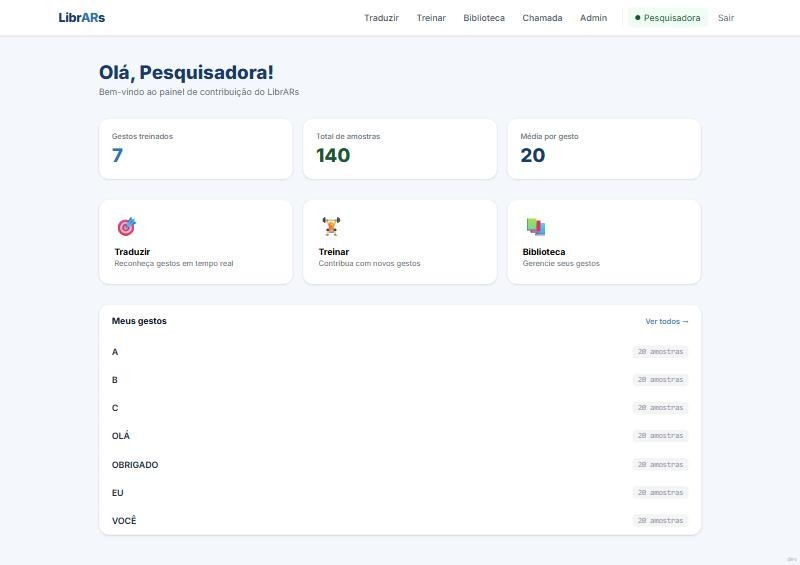
\includegraphics[width=0.85\textwidth]{fig_painel}
\caption{Painel do participante na plataforma LibrARs.}
\label{fig:painel}
\end{figure}

Na tela Treinar, o participante escolhe uma letra do alfabeto ou um sinal comum,
ou digita o nome de um novo gesto, e grava o gesto em frente à câmera. A
plataforma avalia a qualidade da gravação conforme a proporção de quadros em que
a mão foi detectada e orienta o participante a regravar quando a mão sai do quadro
com frequência. Cada gravação armazena até 150 quadros brutos, 20 quadros
amostrados para o classificador estático e um vetor temporal que resume o
movimento.

\begin{figure}[htbp]
\centering
\figpendente{Print da tela Treinar com a câmera ativa: mão detectada, gesto
selecionado e progresso da gravação. (A câmera não pôde ser acessada na captura
automática.)}
\caption{Tela Treinar durante a gravação de um gesto.}
\label{fig:treinar}
\end{figure}

A Biblioteca (Figura~\ref{fig:biblioteca}) lista os gestos do participante e
permite importá-los, exportá-los e carregar a base coletiva, formada pelos gestos
de todos os participantes, para ampliar o vocabulário reconhecido na tradução.

\begin{figure}[htbp]
\centering
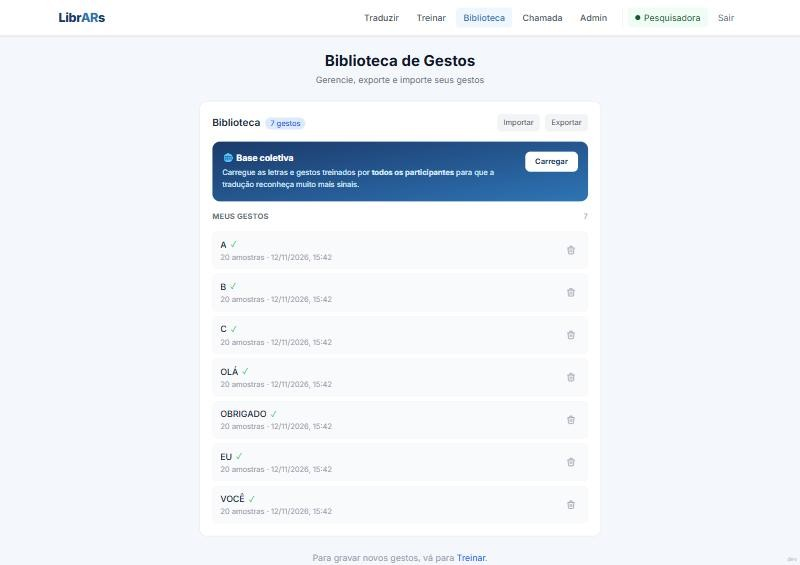
\includegraphics[width=0.85\textwidth]{fig_biblioteca}
\caption{Biblioteca de gestos, com acesso à base coletiva.}
\label{fig:biblioteca}
\end{figure}

A tela Traduzir exibe o gesto reconhecido sobre o vídeo, com uma barra de
confiança (verde a partir de 70\%, amarela entre 45\% e 70\%, vermelha abaixo de
45\%), e acumula os gestos reconhecidos em uma frase. A Chamada
(Figura~\ref{fig:chamada}) permite criar uma sala ou entrar com um código para
uma conversa por vídeo com tradução nos dois sentidos: gestos convertidos em
texto e fala convertida em texto por reconhecimento de voz do navegador.

\begin{figure}[htbp]
\centering
\figpendente{Print da tela Traduzir com a câmera ativa: gesto reconhecido, barra
de confiança e frase detectada.}
\caption{Tela Traduzir reconhecendo um gesto e formando uma frase.}
\label{fig:traduzir}
\end{figure}

\begin{figure}[htbp]
\centering
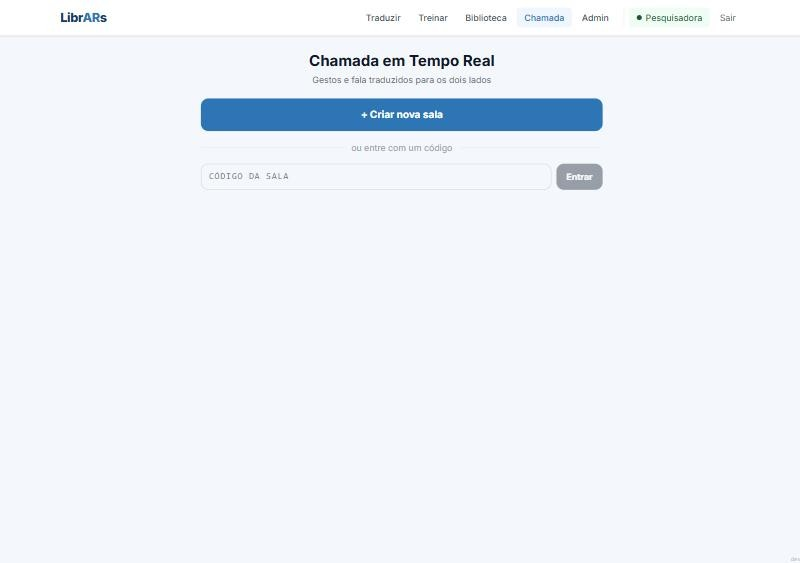
\includegraphics[width=0.85\textwidth]{fig_chamada}
\caption{Tela inicial da chamada em tempo real.}
\label{fig:chamada}
\end{figure}

\subsubsection{Painel do administrador}

O painel do administrador reúne a gestão de participantes
(Figura~\ref{fig:admin-users}), a listagem de todas as gravações
(Figura~\ref{fig:admin-rec}), indicadores de contribuição, a geração de convites
e a exportação do \textit{dataset} bruto em JSON, com os quadros de cada gravação
associados a um identificador do participante. Nas figuras, nomes e e-mails foram
substituídos por identificadores anônimos.

\begin{figure}[htbp]
\centering
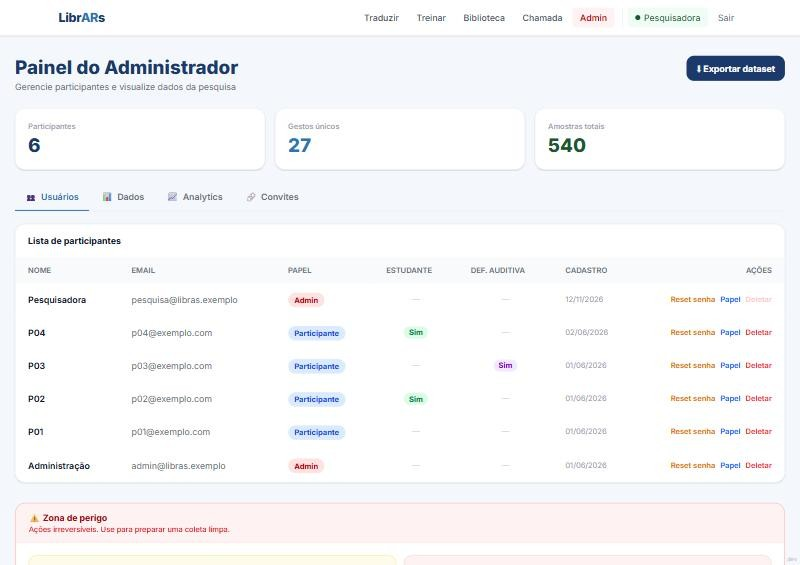
\includegraphics[width=0.9\textwidth]{fig_admin_participantes}
\caption{Painel do administrador: lista de participantes (dados anonimizados).}
\label{fig:admin-users}
\end{figure}

\begin{figure}[htbp]
\centering
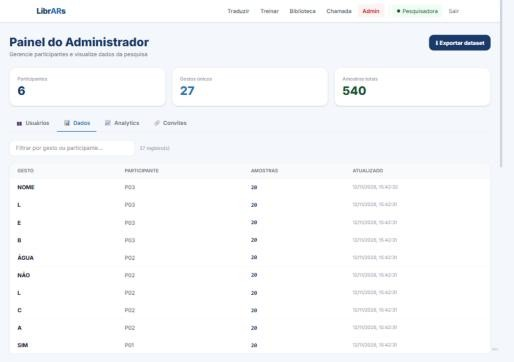
\includegraphics[width=0.75\textwidth]{fig_admin_gravacoes}
\caption{Painel do administrador: gravações por gesto e participante (dados
anonimizados).}
\label{fig:admin-rec}
\end{figure}

\subsubsection{Classificador da plataforma}
\label{subsec:classificador-plataforma}

O reconhecimento na plataforma web não usa a rede CNN + LSTM, e sim um
classificador por $k$ vizinhos mais próximos ($k$-NN) executado no navegador.
Cada quadro é representado pelos 63 valores dos \textit{landmarks}, normalizados
pelo pulso e pela distância pulso–base do dedo médio, como na
Seção~\ref{subsec:pipeline}. A distância entre dois quadros é euclidiana, com peso
0,25 para a coordenada $z$, menos confiável na estimativa monocular. Os 5
vizinhos mais próximos votam com peso inversamente proporcional ao quadrado da
distância, e a predição só é aceita se: (i) o vizinho mais próximo estiver a uma
distância máxima de 1,2; (ii) a confiança do vencedor for de pelo menos 60\%; e
(iii) a diferença para o segundo colocado for de pelo menos 15 pontos percentuais.
Caso contrário, o quadro é rejeitado. Para gestos com movimento, há um caminho
temporal análogo, que compara vetores com média, desvio-padrão, velocidade média
e deslocamento total de cada coordenada ao longo da gravação.

%===================== RESULTADOS E DISCUSSÃO =====================
\section{Resultados e discussão}

\subsection{Métricas de desempenho do modelo}
\label{subsec:metricas-modelo}

Os resultados a seguir foram obtidos com um \textit{dataset} inicial de 2 classes
de gestos (``oi'' e ``obrigado''), após a aplicação dos critérios de exclusão
descritos na Seção~\ref{subsec:coleta}. A Tabela~\ref{tab:metricas} apresenta as
métricas por classe sobre o conjunto de teste.

% [PENDENTE: conferir os números do dataset: o protocolo prevê 10 participantes ×
% 10 repetições (>= 100 amostras por gesto), a versão anterior citava
% "aproximadamente 30 amostras por gesto", e o suporte da tabela soma 38. Informar
% o total de amostras por gesto após a exclusão e quantas foram para treino,
% validação e teste.]

\begin{table}[htbp]
\centering
\caption{Métricas de classificação por classe no conjunto de teste.}
\label{tab:metricas}
\begin{tabular}{@{}l c c c c@{}}
\toprule
\textbf{Gesto} & \textbf{Precisão} & \textbf{Revocação} & \textbf{F1-score} & \textbf{Suporte} \\
\midrule
obrigado & 1,00 & 0,93 & 0,96 & 14 \\
oi & 0,96 & 1,00 & 0,98 & 24 \\
\midrule
Média macro & 0,98 & 0,96 & 0,97 & 38 \\
\addlinespace
\multicolumn{4}{@{}l}{Acurácia global} & 97,4\% \\
\multicolumn{4}{@{}l}{Kappa de Cohen} & 0,94 \\
\bottomrule
\end{tabular}
\end{table}

Complementarmente, o modelo obteve F1 macro de 0,97 e coeficiente Kappa de Cohen
de 0,94, indicando concordância quase perfeita entre as predições do modelo e os
rótulos reais: segundo a escala de interpretação de Landis e Koch (1977), valores
de Kappa entre 0,81 e 1,00 correspondem a concordância quase perfeita.

\begin{figure}[htbp]
\centering
\figpendente{Inserir a imagem gerada por \texttt{evaluate\_model.py} (pasta
\texttt{logs/} ou equivalente).}
\caption{Matriz de confusão do modelo no conjunto de teste.}
\label{fig:cm-modelo}
\end{figure}

\begin{figure}[htbp]
\centering
\figpendente{Inserir o gráfico gerado a partir do \texttt{CSVLogger}
(\texttt{logs/training\_log.csv} ou equivalente).}
\caption{Curvas de acurácia e perda de treinamento e validação ao longo das
épocas.}
\label{fig:curvas}
\end{figure}

\subsection{Discussão dos resultados}

O resultado de 97,4\% de acurácia é expressivo e está em linha com trabalhos
recentes da área — a título de comparação, o sistema de reconhecimento de sílabas
em Libras listado na Tabela~\ref{tab:relacionados} reporta exatamente o mesmo
valor de acurácia média em condições controladas, ainda que sobre vocabulário e
\textit{dataset} distintos. Também é superior ao reportado por Rego et al.\ (2025)
no \textit{dataset} MINDS-Libras (92\%), embora essa comparação deva ser lida com
cautela, pois os \textit{datasets}, o número de classes e a metodologia de
validação não são idênticos.

É necessário, no entanto, interpretar esse número com cautela metodológica. O
conjunto avaliado contém apenas 2 classes e 38 amostras de teste — uma base de
dados consideravelmente menor do que a de trabalhos de referência da área, como o
MINDS-Libras, que reúne 1.155 vídeos cobrindo 20 sinais executados por 12
sinalizantes (REZENDE; ALMEIDA; GUIMARÃES, 2021). \textit{Datasets} pequenos
aumentam o risco de \textit{overfitting}: é possível que o modelo esteja
memorizando particularidades dos poucos sinalizantes presentes no treinamento, em
vez de aprender um padrão de gesto generalizável. Esse risco é discutido de forma
mais detalhada na Seção~\ref{subsec:limitacoes}.

Com a ampliação planejada do \textit{dataset} — para 60 a 100 amostras por gesto,
maior número de participantes e inclusão de vocabulário relacionado à área de
computação (ver Seção~\ref{subsec:futuros}) — espera-se manter ou aproximar essa
acurácia sob condições de avaliação mais rigorosas, notadamente com validação em
dados de usuários não presentes no treinamento.

\subsection{Dados coletados na plataforma web}

Até a data desta versão, a plataforma registra 6 participantes cadastrados, dos
quais 4 contribuíram com gravações, todas realizadas entre 2 e 4 de junho de
2026. A Tabela~\ref{tab:composicao} resume o \textit{dataset} exportado, e a
Figura~\ref{fig:quadros-part} mostra a contribuição de cada participante.

\begin{table}[htbp]
\centering
\caption{Composição do dataset da plataforma web.}
\label{tab:composicao}
\begin{tabular}{@{}l c@{}}
\toprule
\textbf{Item} & \textbf{Valor} \\
\midrule
Participantes cadastrados & 6 \\
Participantes com gravações & 4 \\
Participantes com deficiência auditiva declarada & 0 \\
Gravações (gesto $\times$ participante) & 30 \\
Gestos distintos & 23 \\
Gestos gravados por mais de um participante & 5 (A, B, C, E, L) \\
Quadros brutos (até 150 por gravação) & 3.481 \\
Quadros amostrados para o classificador & 597 \\
\bottomrule
\end{tabular}
\end{table}

Cada gesto de cada participante corresponde a uma única gravação; as ``20
amostras'' exibidas na plataforma são quadros dessa gravação, e não repetições
independentes do gesto. Por isso, o \textit{dataset} ainda não atende ao
protocolo de 10 repetições por gesto descrito na Seção~\ref{subsec:coleta}.

\begin{figure}[htbp]
\centering
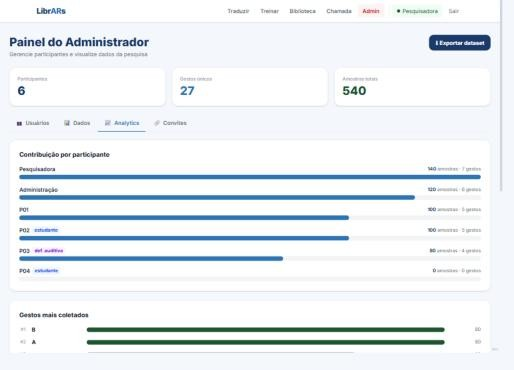
\includegraphics[width=0.75\textwidth]{fig_contribuicao}
\caption{Quadros amostrados e gestos gravados por participante.}
\label{fig:quadros-part}
\end{figure}

\subsection{Avaliação do classificador da plataforma web}

O classificador descrito na Seção~\ref{subsec:classificador-plataforma} foi
avaliado sobre o \textit{dataset} exportado, reproduzindo a mesma regra de decisão
e os mesmos limiares usados em produção. A avaliação é feita por quadro e
considera três desfechos: acerto, erro (outro gesto aceito) ou rejeição. Foram
usados dois cenários:

\begin{itemize}[leftmargin=2cm]
  \item \textbf{Mesmo sinalizante:} para as 19 gravações do participante P01, a
  primeira metade dos quadros de cada gravação serve de referência e a segunda
  metade é classificada. Como os quadros vêm da mesma gravação, este cenário é
  otimista;
  \item \textbf{Sinalizante excluído} (\textit{leave-one-participant-out}): os
  quadros de cada participante são classificados usando como referência apenas as
  gravações dos demais. Só entram os gestos que outro participante também gravou
  (A, B, C, E e L).
\end{itemize}

\begin{table}[htbp]
\centering
\caption{Desempenho do classificador da plataforma, por quadro.}
\label{tab:desempenho-plataforma}
\begin{tabular}{@{}l c c@{}}
\toprule
 & \textbf{Mesmo sinalizante} & \textbf{Sinalizante excluído} \\
\midrule
Quadros avaliados & 1.383 & 1.319 \\
Gestos & 19 & 5 \\
Acertos & 72,5\% & 35,5\% \\
Erros & 13,5\% & 9,9\% \\
Rejeitados & 14,0\% & 54,7\% \\
Precisão entre os aceitos & 84,3\% & 78,3\% \\
\bottomrule
\end{tabular}
\end{table}

No cenário de mesmo sinalizante (Figura~\ref{fig:cm-mesmo}), 11 dos 19 gestos
superam 85\% de acerto. As falhas se concentram em pares de configuração de mão
semelhante: B é confundido com F, S com MULHER e V com U; C, E e L são
majoritariamente rejeitados.

Com o sinalizante excluído (Figuras~\ref{fig:cm-excluido} e~\ref{fig:acerto-part}),
o acerto cai para 35,5\%, e a maior parte dos quadros é rejeitada, e não
classificada errado: o classificador tende a abster-se diante de uma mão que não
conhece. A exceção é a letra A, confundida com MULHER em 43\% dos quadros. O
desempenho também varia muito entre participantes, de 0\% a 82\%.

\begin{figure}[htbp]
\centering
\figpendente{Matriz de confusão do classificador da plataforma no cenário de
mesmo sinalizante (participante P01).}
\caption{Matriz de confusão do classificador da plataforma no cenário de mesmo
sinalizante (participante P01).}
\label{fig:cm-mesmo}
\end{figure}

\begin{figure}[htbp]
\centering
\figpendente{Matriz de confusão no cenário de sinalizante excluído.}
\caption{Matriz de confusão no cenário de sinalizante excluído.}
\label{fig:cm-excluido}
\end{figure}

\begin{figure}[htbp]
\centering
\figpendente{Gráfico de barras: acerto por participante no cenário de sinalizante
excluído.}
\caption{Acerto por participante no cenário de sinalizante excluído.}
\label{fig:acerto-part}
\end{figure}

Por fim, os 2.162 quadros de gestos que não existiam na referência do cenário de
sinalizante excluído permitem medir o comportamento diante de sinais
desconhecidos: 77,8\% foram corretamente rejeitados, mas 22,2\% foram aceitos
como algum outro gesto.

Esses resultados confirmam, com dados reais da plataforma, a limitação de
generalização discutida na Seção~\ref{subsec:limitacoes}: o reconhecimento
funciona bem para quem gravou o gesto, mas ainda não para novos usuários. A
avaliação considera apenas o caminho estático do classificador e quadros
isolados; o desempenho percebido na tela Traduzir, que acumula decisões ao longo
do tempo, pode ser diferente.

\subsection{Resultados da validação com usuários}

% [PENDENTE: seção a ser preenchida após as sessões descritas na
% Seção 4.6. Conteúdo previsto: tabela de caracterização dos participantes
% (anonimizada), acurácia por participante, matriz de confusão agregada, tempo
% médio até o reconhecimento e síntese do questionário de percepção.]

\begin{figure}[htbp]
\centering
\figpendente{Gráfico de barras: participantes P01–P05 no eixo $x$, acurácia no
eixo $y$, com linha de referência na acurácia do conjunto de teste original.}
\caption{Acurácia de reconhecimento por participante na validação.}
\label{fig:acuracia-validacao}
\end{figure}

\begin{figure}[htbp]
\centering
\figpendente{Gráfico de barras empilhadas por item do questionário (escala de 1 a
5).}
\caption{Respostas ao questionário de percepção.}
\label{fig:questionario}
\end{figure}

\subsection{Limitações}
\label{subsec:limitacoes}

Apesar dos resultados preliminares expressivos, este trabalho apresenta
limitações que devem ser consideradas na interpretação dos resultados e no
planejamento das próximas etapas:

\begin{itemize}[leftmargin=2cm]
  \item \textbf{Tamanho reduzido do \textit{dataset}:} os resultados atuais foram
  obtidos com apenas 2 classes de gestos e um número limitado de amostras, o que
  aumenta o risco de \textit{overfitting} e limita a generalização das métricas
  reportadas;
  \item \textbf{Ausência de validação com usuário externo ao treinamento:} até a
  realização da validação descrita na Seção~\ref{subsec:validacao}, o modelo não
  foi testado com dados de um participante ausente do conjunto de treinamento —
  etapa necessária para confirmar a real capacidade de generalização do sistema,
  e que trabalhos comparáveis da literatura (MOREIRA, 2026) também apontam como
  necessária;
  \item \textbf{Dificuldades técnicas observadas:} mãos parcialmente fora do
  quadro de captura, movimentos executados em alta velocidade e gestos
  visualmente semelhantes representaram os principais desafios para o
  rastreamento e a classificação corretos;
  \item \textbf{Escopo restrito às mãos:} o sistema atual não incorpora
  expressões não-manuais (expressão facial, movimento de cabeça e tronco), que
  cumprem funções gramaticais na Libras (QUADROS; KARNOPP, 2004) e cuja ausência
  limita o reconhecimento a um subconjunto do que a língua efetivamente expressa;
  \item \textbf{Perfil dos participantes da coleta:} as amostras de treinamento
  foram coletadas sem a participação de pessoas surdas ou intérpretes de Libras, o
  que pode afetar a precisão linguística dos gestos aprendidos pelo modelo.
  % [PENDENTE: confirmar quem foram os 10 participantes da coleta, para manter
  % este item coerente com a Seção 4.2.]
\end{itemize}

\subsection{Trabalhos futuros}
\label{subsec:futuros}

Como desdobramentos deste trabalho, planeja-se:

\begin{itemize}[leftmargin=2cm]
  \item expandir o \textit{dataset} com gestos relacionados à área de computação,
  ampliando o vocabulário reconhecido pelo sistema;
  \item ampliar a validação de generalização com mais usuários não presentes no
  conjunto de treinamento, seguindo protocolo \textit{signer-independent}
  semelhante ao adotado em trabalhos recentes da área;
  \item incorporar expressões não-manuais ao \textit{pipeline} de reconhecimento,
  ampliando a cobertura gramatical do sistema;
  \item dar continuidade à pesquisa em nível de mestrado, com possível publicação
  dos resultados em artigo científico.
\end{itemize}

%====================== CONSIDERAÇÕES FINAIS ======================
\section{Considerações finais}

Este trabalho apresentou o desenvolvimento do LibrasAI, um sistema de
reconhecimento automático de gestos dinâmicos de Libras em tempo real, construído
a partir de um \textit{pipeline} que integra captura de vídeo, extração de
\textit{landmarks} via MediaPipe, normalização espacial e classificação por meio
de uma rede híbrida CNN + LSTM.

Os objetivos específicos definidos para este estágio do trabalho foram
majoritariamente alcançados: o \textit{pipeline} de captura e detecção de
\textit{landmarks} está implementado e em funcionamento; o modelo CNN + LSTM foi
treinado e superou a meta de acurácia estabelecida (90\%), atingindo 97,4\% sobre
o \textit{dataset} inicial; o sistema de coleta interativa de dados está
operacional e já produziu um protocolo replicável com 10 participantes; e a
formação automática de frases, com os três modos de operação planejados, foi
implementada e testada pela equipe de desenvolvimento.

Ao mesmo tempo, este trabalho reconhece explicitamente que os resultados obtidos
são preliminares e devem ser lidos à luz das limitações discutidas na
Seção~\ref{subsec:limitacoes} — em especial o tamanho ainda reduzido do
\textit{dataset} e a necessidade de validação com usuários externos ao
treinamento, endereçada pelo protocolo descrito na Seção~\ref{subsec:validacao}.
Essas limitações não invalidam a contribuição do trabalho, mas delimitam com
precisão o que ainda precisa ser feito antes que o sistema possa ser considerado
robusto o suficiente para uso real pela comunidade surda.

Do ponto de vista de contribuição acadêmica, o LibrasAI se soma a um conjunto
ainda pequeno de sistemas de reconhecimento de Libras — em contraste com a
abundância de trabalhos voltados à ASL e a outras línguas de sinais
internacionais —, reforçando a relevância de pesquisa nacional dedicada
especificamente à língua de sinais brasileira. A intenção declarada de dar
continuidade a este trabalho em nível de mestrado, com submissão dos resultados a
um artigo científico, indica que o presente TCC deve ser compreendido como uma
etapa inicial de um programa de pesquisa mais amplo, e não como um produto
finalizado.


%=================== ELEMENTOS PÓS-TEXTUAIS ===================
%========================== REFERÊNCIAS ==========================
\newpage
\section*{Referências}
\addcontentsline{toc}{section}{REFERÊNCIAS}

\begingroup
\singlespacing
\setlength{\parindent}{0pt}
\setlength{\parskip}{0.7\baselineskip}

BRASIL. \textbf{Lei n. 10.436, de 24 de abril de 2002}. Dispõe sobre a Língua
Brasileira de Sinais – Libras e dá outras providências. Diário Oficial da União:
Brasília, DF, 2002.

BRASIL. \textbf{Decreto n. 5.626, de 22 de dezembro de 2005}. Regulamenta a Lei
n. 10.436, de 24 de abril de 2002. Diário Oficial da União: Brasília, DF, 2005.

HOCHREITER, S.; SCHMIDHUBER, J. Long short-term memory. \textbf{Neural
Computation}, v. 9, n. 8, p. 1735--1780, 1997.

IBGE. [PENDENTE: referência completa da fonte do dado de 10 milhões de pessoas
com deficiência auditiva (pesquisa, ano e \textit{link})]

LANDIS, J. R.; KOCH, G. G. The measurement of observer agreement for categorical
data. \textbf{Biometrics}, v. 33, n. 1, p. 159--174, 1977.

MEDIAPIPE. \textbf{MediaPipe Hands Solution}. Google LLC. Disponível em:
\url{https://developers.google.com/mediapipe/solutions/vision/hand_landmarker}.
Acesso em: [PENDENTE: data].

MOREIRA, J. \textbf{Dynamic LIBRAS gesture recognition via CNN over spatiotemporal
matrix representation}. Curitiba: Universidade Tecnológica Federal do Paraná,
2026. Disponível em: arXiv:2603.25863.

PIGOU, L. et al. Beyond temporal pooling: recurrence and temporal convolutions
for gesture recognition in video. \textbf{International Journal of Computer
Vision}, v. 126, n. 2--4, p. 430--439, 2018.

[PENDENTE: referência completa do trabalho de reconhecimento de sílabas em Libras
para HRI (2026) citado na Tabela~\ref{tab:relacionados}]

QUADROS, R. M. de. \textbf{Libras}. São Paulo: Parábola, 2019. (Linguística para
o ensino superior).

QUADROS, R. M. de; KARNOPP, L. B. \textbf{Língua de sinais brasileira}: estudos
linguísticos. Porto Alegre: Artmed, 2004.

REGO, T. et al. Brazilian sign language recognition using deep learning based on
fast Fourier transform and kinematic features. \textbf{IEEE Access}, 2025.

REZENDE, T. M.; ALMEIDA, S. G. M.; GUIMARÃES, F. G. \textbf{Reconhecimento
automático de sinais da Libras}: desenvolvimento da base de dados MINDS-Libras e
modelos de redes neurais convolucionais. Tese (Doutorado em Engenharia Elétrica)
– Universidade Federal de Minas Gerais, Belo Horizonte, 2021.

RONCHETTI, F. et al. LSA64: an Argentinian sign language dataset. In: CONGRESO
ARGENTINO DE CIENCIAS DE LA COMPUTACIÓN, 22., 2016. \textbf{Actas} [...]. 2016.

SINCAN, O. M.; KELES, H. Y. AUTSL: a large scale multi-modal Turkish sign
language dataset and baseline methods. \textbf{IEEE Access}, v. 8, p.
181340--181355, 2020.

TENSORFLOW. \textbf{TensorFlow documentation}: Keras LSTM layer. Disponível em:
\url{https://www.tensorflow.org/api_docs/python/tf/keras/layers/LSTM}. Acesso em:
[PENDENTE: data].

ZHANG, F. et al. MediaPipe Hands: on-device real-time hand tracking. In: CVPR
WORKSHOP ON COMPUTER VISION FOR AUGMENTED AND VIRTUAL REALITY, 2020.
\textbf{Proceedings} [...]. 2020.
\endgroup


\end{document}
